\section{Risultati}
L'applicazione dell'indice a ogni immagine Sentinel-2 e il calcolo della percentuale di celle innevate consentono di stimare la quota di neve (definita come la fascia innevata più bassa) per ogni data di acquisizione.
\begin{table}[H] \centering
    \caption{Tabella riassuntiva del lavoro, indicante la quota delle nevi per ogni data di acquisizione, con un riferimento alla percentuale di copertura nuvolosa.}
\begin{tabular}{ccc}
    \toprule
           & Snow line (m s.l.m.) & Cop. nuvolosa (\%) \\
    \midrule
02/05/2025 & 2260       & 7     \\
30/05/2025 & 2460       & 1     \\
09/06/2025 & 2680       & 0     \\
13/06/2025 & 2800       & 0     \\
19/06/2025 & 3060       & 33    \\
09/07/2025 & 3060       & 4     \\
08/08/2025 & 3280       & 1     \\
13/08/2025 & 3280       & 2     \\
18/08/2025 & 3280       & 2     \\
25/08/2025 & 3320       & 0     \\
17/09/2025 & 3280       & 7     \\
19/09/2025 & 3280       & 0     \\
29/09/2025 & 2600       & 0     \\
        \midrule
\end{tabular}
\end{table}
Come descritto nella sezione relativa a materiali e metodi, la copertura nuvolosa (pur estesa, come verificatosi il 19/06/2025) non ha inficiato l'applicazione dell'indice, poiché ha interessato esclusivamente le zone a quote inferiori.
\begin{figure}[H]
    \centering
    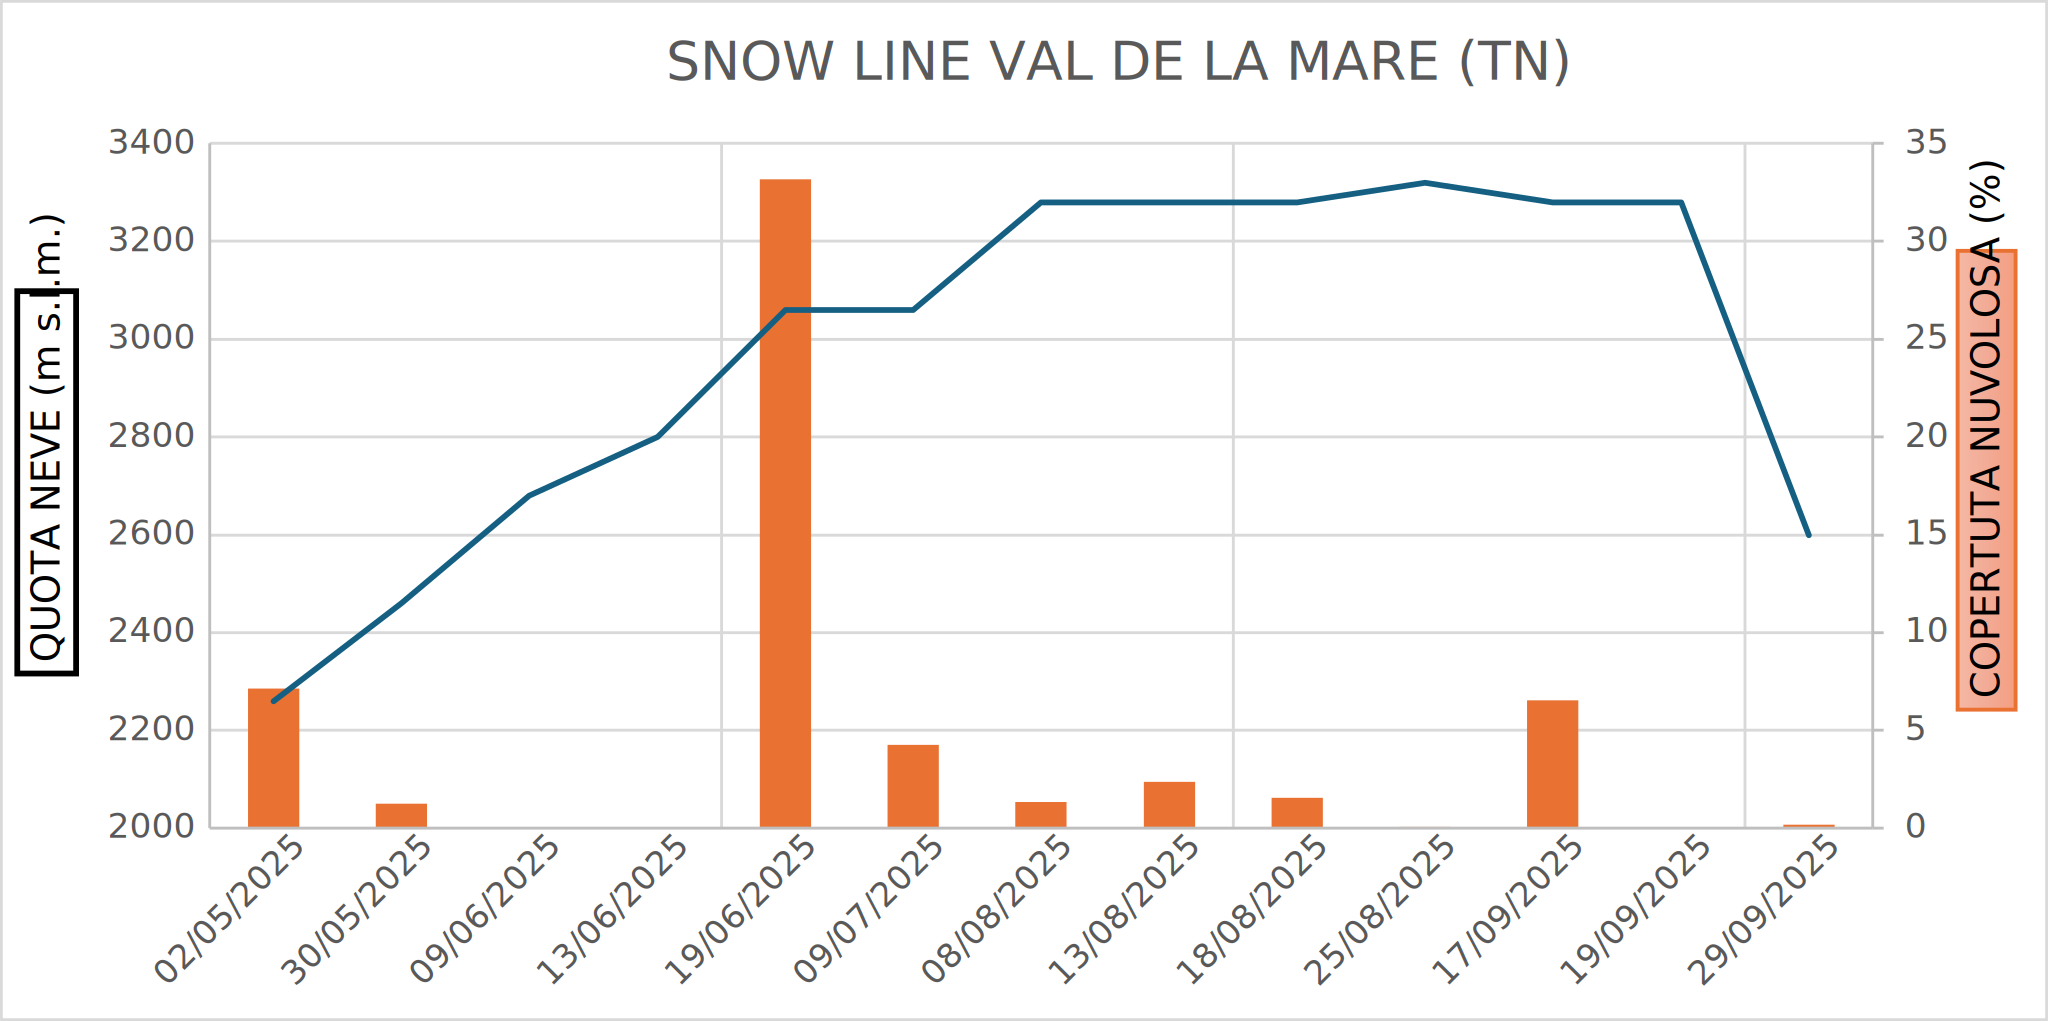
\includegraphics[width=0.7\textwidth]{immagini/sl_valdelamare.png}
    \caption{Linea della neve, nel periodo estivo 2025, nella Val de la Mare (TN).}
    \label{fig:sl_valdelamare}
\end{figure}

\begin{figure}[H]
     \centering
     % Prima immagine
     \begin{subfigure}[b]{0.6\textwidth}
         \centering
         \includegraphics[width=\textwidth]{immagini/sl_30_05_2025.pdf}
         \caption{30/05/2025 (2460 m s.l.m.)}
         \label{fig:img1}
     \end{subfigure}
     \hfill % Spazio elastico per distribuire le immagini
     % Seconda immagine
     \begin{subfigure}[b]{0.6\textwidth}
         \centering
         \includegraphics[width=\textwidth]{immagini/sl_13_06_2025.pdf}
         \caption{13/06/2025 (2800 m s.l.m.)}
         \label{fig:img2}
     \end{subfigure}
     \hfill % Spazio elastico
     % Terza immagine
     \begin{subfigure}[b]{0.6\textwidth}
         \centering
         \includegraphics[width=\textwidth]{immagini/sl_17_09_2025.pdf}
         \caption{17/09/2025 (3280 m s.l.m.)}
         \label{fig:img3}
     \end{subfigure}
     
     \caption{Isopse (a 20 metri) indicanti le condizioni di innevamento al suolo della Val de la Mare. Le fasce rosse rappresentano le aree considerate innevate, mentre quelle verdi rappresentano una condizione di non innevamento. In tutte e tre le immagini, l'immagine sullo sfondo è un rilievo di Google Satellite.}
     \label{fig:tre_immagini_compatte}
\end{figure}